\subsection{Vector-Valued Functions}
%
\BEN 
%% ~~~~~~~~~~~~~~~~~~~~~~~~~~~~~~~~~~~~~~~~~~~~~~~~~~~~~~~~~~~~~~~~~~~~~~~~~~~~~~~~~
%\item 
%Use row-reduction operations on the augmented matrices.
%\begin{align}
% \begin{amatrix}{4}
%  1 & 2 & 0 & 1 & 1 \\
%  3 & -1 & 1 & 2 & 5 \\
%  0 & 1 & 0 & 2 & 0 \\
%  4 & 0 & 3 & 1 & 10
% \end{amatrix}&
% \nonumber \\
% \begin{amatrix}{4}
%  1 & 2 & 0 & 1 & 1 \\
%  0 & -7 & 1 & -1 & 2 \\
%  0 & 1 & 0 & 2 & 0 \\
%  0 & -8 & 3 & -3 & 6
% \end{amatrix}&
% \begin{array}{l}
%  R_2 \leftarrow R_2 - 3R_1 \\ R_4 \leftarrow R_4 - 4R_1 
% \end{array}
% \nonumber \\
% \begin{amatrix}{4}
%  1 & 2 & 0 & 1 & 1 \\
%  0 & 0 & 1 & 13 & 2 \\
%  0 & 1 & 0 & 2 & 0 \\
%  0 & 0 & 3 & 13 & 6
% \end{amatrix}&
% \begin{array}{l}
%  R_2 \leftarrow R_2 + 7R_3 \\ R_4 \leftarrow R_4 + 8R_3
% \end{array}
% \nonumber \\
% \begin{amatrix}{4}
%  1 & 2 & 0 & 1 & 1 \\
%  0 & 0 & 1 & 13 & 2 \\
%  0 & 1 & 0 & 2 & 0 \\
%  0 & 0 & 0 & -26 & 0
% \end{amatrix}&
% \begin{array}{l}
%  R_4 \leftarrow R_4 - 3R_2
% \end{array}
% \nonumber
%\end{align}
%
%This is equivalent to the system of equations
%
%\begin{align}
% x + 2y + w &= 1 \nonumber \\
% z + 13w &= 2 \nonumber \\
% y + 2w &= 0 \label{q2_a:a} \\
% -26w &= 0 \label{q2_a:b}
%\end{align}
%
%Equations (\ref{q2_a:a}) and (\ref{q2_a:b}) show that $w = 0$ and
%$y = 0$, and substitution yields $z = 2$ and $x = 1$.
%
%% ~~~~~~~~~~~~~~~~~~~~~~~~~~~~~~~~~~~~~~~~~~~~~~~~~~~~~~~~~~~~~~~~~~~~~~~~~~~~~~~~~
%\item
%\BEN
%\item
%It's not possible to calculate the determinant of $A$, because $A$ is not square. We can however solve $A\mathbf{x}=\mathbf{b}$ for \textbf{x} using row operations:
%\begin{align}
% \begin{amatrix}{4}
%  -3 &  1 & 2 &  4 & 1 \\
%   2 & -1 & 2 &  3 & 1 \\
%   1 &  0 & 4 & -2 & 1
% \end{amatrix}&
% \nonumber \\
% \begin{amatrix}{4}
%  0 &  1 & 14 & -2 &  4 \\
%  0 & -1 & -6 &  7 & -1 \\
%  1 &  0 &  4 & -2 &  1
% \end{amatrix}&
% \begin{array}{l}
%  R_1 \leftarrow R_1 + 3R_3 \\ R_2 \leftarrow R_2 - 2R_3
% \end{array}
% \nonumber \\
% \begin{amatrix}{4}
%  0 & 1 & 14 & -2 & 4 \\
%  0 & 0 &  8 &  5 & 3 \\
%  1 & 0 &  4 & -2 & 1
% \end{amatrix}&
% \begin{array}{l}
%  R_2 \leftarrow R_2 + R_1
% \end{array}
% \nonumber
%\end{align}
%
%This is equivalent to the system of equations
%
%\begin{align}
% y + 14z -2w &= 4 \label{asdfasdf} \\
% 8z + 5w &= 3 \label{qwerqwer} \\
% x + 4z -2w &= 1 \label{zxcvzxcv}
%\end{align}
%
%Since there are fewer equations than unknowns we will parameterize the 
%solution set by setting $w = t$, where $t$ is any real number.  From equation 
%(\ref{qwerqwer}) we get $z = \frac{3}{8} - \frac{5}{8}t$.  Substituting $z$ into 
%equations (\ref{zxcvzxcv}) and (\ref{asdfasdf}) yields $x = -\frac{1}{2} + 
%\frac{9}{2}t$ and $y = -\frac{5}{4} + \frac{43}{4}t$. \\
%
%Because of the free parameter $t$, there are infinitely many solutions to the given system.
%% ~  ~  ~  ~  ~  ~  ~  ~  ~  ~  ~  ~  ~  ~  ~  ~  ~  ~  ~  ~  ~  ~  ~  ~  ~  ~  ~  ~  ~  ~  ~  ~  ~  ~  ~  ~  
%\item
%We can calculate the 3$\times$3 determinant by expanding into 2$\times$2 determinants:
%\begin{align*}
% \begin{vmatrix}
%  1 &  2 & -1 \\
%  2 &  5 &  0 \\
% 4 & 9 &  -2
% \end{vmatrix} &=
% 1 \begin{vmatrix} 5 & 0 \\ 9 & -2 \end{vmatrix}
% -2 \begin{vmatrix} 2 & 0 \\ 4 & -2 \end{vmatrix}
% -1 \begin{vmatrix} 2 & 5 \\ 4 & 9 \end{vmatrix} \\
% &= (-10) -2 (-4) -(18 - 20) \\
% &= -10 + 8 + 2 \\
% &= 0
%\end{align*}
%Applying one row operation yields
%\begin{align*}
% \begin{amatrix}{3}
%  1 & 2 & -1  & 1 \\
%  2 & 5 & 0 & 5 \\
%  4 & 9 & -2 & 0 
% \end{amatrix} \sim
%  \begin{amatrix}{3}
%  1 & 2 & -1  & 1 \\
%  2 & 5 & 0 & 5 \\
%  0 & 0 & 0 & -7
% \end{amatrix}
%  \begin{array}{l}
%  \\ \\
%  R_3 \leftarrow R_3 - 2R_1 - R_2  \
% \end{array}
% \end{align*}
% The last row is equivalent to 
% \begin{align*}
%0x+0y+0z = -7,
%\end{align*}
%which implies that this particular system has no solution. 
% % ~~~~~~~~~~~~~~~~~~~~~~~~~~~~~~~~~~~~~~~~~~~~~~~~~~~~~~~~~~~~~~~~~~~~~~~~~~~~~~~~~
%\EEN

\item The derivative of $\textbf{r}$ is simply
\(
  \mathbf{r}'(t) = 2t \mathbf{i} + \mathbf{j}.
\)

\BEN
\item \(
  \mathbf{r}(t) \perp  \mathbf{r}'(t)
\)
implies
\begin{align*}
  0& = \mathbf{r}(t) \cdot  \mathbf{r}'(t) \\
  &= \big((1+t^2) \mathbf{i} + t\mathbf{j} \big) \cdot \big(2t \mathbf{i} + \mathbf{j}\big) \\
  &= (2t+2t^3) + (t)\\
  &= t(3+2t^2)
\end{align*}
This equation is satisfied only when $t=0$ or $t^2 = -3/2$. The latter equation cannot be satisfied if $t\in\R$. Thus, the two vectors are only perpendicular when $t=0$. Thus,  \(\mathbf{r}(t)\) is perpendicular to \(\mathbf{r}'(t)\) at (0,1). 
\item If \(\mathbf{r}(t)\) is pointing in the same direction as \(\mathbf{r}'(t)\), then \ \(\mathbf{r}(t) = C  \mathbf{r}'(t)\), where $C$ is a positive constant. Equating the components of the vectors yields the two equations
\begin{align*}
  (1+t^2)& = C2t , \text{ and } t=C.
\end{align*}
If we substitute $t=C$ into the first equation, we find
\begin{align*}
  (1+C^2)& = 2C^2\\
  C&=+1,
\end{align*}
because $C$ must be positive. Thus, the two vectors are pointing in the same direction when $t=1$, which is at the point (2,1).
\item
The solution is the similar to part (b), except that $C$ must be a negative constant. We find that the vectors point in opposite directions when $C=t=-1$, and at the point (2,-1).
\EEN
% ~~~~~~~~~~~~~~~~~~~~~~~~~~~~~~~~~~~~~~~~~~~~~~~~~~~~~~~~~~~~~~~~~~~~~~~~~~~~~~~~~

%\item
%We first convert the system of equations into an equivalent augmented-matrix
%form:
%\[
% \begin{amatrix}{3}
%  1 & 2 & -1 & 2 \\
%  2 & a & -2 & b \\
%  3 & 2 & 0 & 1
% \end{amatrix}.
%\]
%Then apply a sequence of row-reduction operations:
%\begin{align}
% \begin{amatrix}{3}
%  1 &   2 & -1 &   2 \\
%  0 & a-4 &  0 & b-4 \\
%  0 &  -4 &  3 &  -5
% \end{amatrix} &  \nonumber \\
% \begin{amatrix}{3}
%  1 &  2 & -1 &   2 \\
%  0 &  a & -3 & b+1 \\
%  0 & -4 &  3 &  -5
% \end{amatrix} & \begin{array}{l} R_2 - 2R_1 \\ R_3 - 3R_1 \end{array} 
% \nonumber \\
% \begin{amatrix}{3}
%  1 & 2 & -1 &   2 \\
%  0 & a & -3 & b+1 \\
%  0 & 4 & -3 &   5
% \end{amatrix} &  \begin{array}{l} R_2 - R_3 \end{array}
% \nonumber \\
% \begin{amatrix}{3}
%  1 & 2 & -1 &   2 \\
%  0 & 4 & -3 &   5 \\
%  0 & a & -3 & b+1
% \end{amatrix} &\begin{array}{l} -1 \cdot R_3 \\ R_2 \leftrightarrow R_3 \end{array}
% \label{eq:reduced}
%\end{align}
%
%Suppose that $a = 4$.  Then (\ref{eq:reduced}) becomes
%\begin{align}
% \begin{amatrix}{3}
%  1 & 2 & -1 &   2 \\
%  0 & 4 & -3 &   5 \\
%  0 & 4 & -3 & b+1
% \end{amatrix} &
% \nonumber \\
% \begin{amatrix}{3}
%  1 & 2 & -1 &   2 \\
%  0 & 4 & -3 &   5 \\
%  0 & 0 &  0 & b-4
% \end{amatrix}&  \begin{array}{l} R_3 - R_2 \end{array}
% \label{eq:substitute_a}
%\end{align}
%
%If $b \neq 4$, then the system has no solutions, since the last row is
%equivalent to the equation $0 = b-4$ where $b-4 \neq 0$.  Conversely, if
%$b = 4$, then (\ref{eq:substitute_a}) is equivalent to the system of
%equations
%\begin{align*}
% x + 2y -z &= 2 \\
% 4y - 3z &= 5
%\end{align*}
%There are fewer equations than unknowns, so we have to parameterize the
%solution set; let $z = t$.  Solving these two equations yields the solution
%\begin{equation}\begin{aligned}
% x &= -\frac{1}{2} - \frac{1}{2}t \\
% y &= \frac{5}{4} + \frac{3}{4}t \\
% z &= t
%\end{aligned}\label{q4:inf}\end{equation}
%
%Now suppose that $a = 0$.  Then the matrix (\ref{eq:reduced}) is equivalent
%to the system
%
%\begin{align*}
% x + 2y -z &= 2 \\
% 4y -3z &= 5 \\
% -3z &= b+1
%\end{align*}
%
%Using back-substitution we find that
%
%\begin{equation}\begin{aligned}
% x &= -\frac{1}{3} - \frac{1}{6}b \\
% y &= 1 - \frac{1}{4}b \\
% z &= \frac{-1}{3} - \frac{1}{3}b
%\end{aligned}\label{q4:a_zero}\end{equation}
%
%Now suppose that $a \neq 4$ and $a \neq 0$.  Then we can continue row-
%reducing from (\ref{eq:reduced}):
%
%\begin{align}
% \begin{amatrix}{3}
%  1 & 2 & -1 &   2 \\
%  0 & 4 & -3 &   5 \\
%  0 & a & -3 & b+1
% \end{amatrix} &
% \nonumber \\
% \begin{amatrix}{3}
%  1 & 2 & -1 & 2 \\
%  0 & 4 & -3 & 5 \\
%  0 & 0 & -3 + \frac{3}{4}a & 1 + b - \frac{5}{4}a
% \end{amatrix}&
% \begin{array}{l}
%  R_3 \leftarrow R_3 - \dfrac{a}{4}R_2
% \end{array} 
% \nonumber
%\end{align}
%
%This is equivalent to the system
%
%\begin{align*}
% x + 2y - z &= 2 \\
% 4y -3z &= 5 \\
% (-3 + \frac{3}{4}a)z &= 1 + b - \frac{5}{4}a
%\end{align*}
%
%Let $c = \dfrac{1 + b - \frac{5}{4}a}{-3 + \frac{3}{4}a}$.  Using back-substitution we find the solution
%
%\begin{equation}\begin{aligned}
% x &= -\frac{1}{2} - \frac{1}{2}c \\
% y &= \frac{5}{4} + \frac{3}{4}c \\
% z &= c
%\end{aligned}\label{q4:one}\end{equation}
%
%Thus we have shown that:
%\begin{enumerate}
%\item When $a = 4$ and $b = 4$ there are infinitely many solutions, given
%by the parameterization (\ref{q4:inf}).
%\item When $a = 4$ and $b \neq 4$ there are no solutions.
%\item When $a \neq 4$ there is one solution.  When $a = 0$, the 
%solution (\ref{q4:a_zero}) is equivalent to that of (\ref{q4:one}).  
%So the solution when $a \neq 4$ is given by (\ref{q4:one}).
%\end{enumerate}
% ~~~~~~~~~~~~~~~~~~~~~~~~~~~~~~~~~~~~~~~~~~~~~~~~~~~~~~~~~
% TORQUE, PARTICLE MOTION
\item
\BEN
\item Differentiating the equation for angular momentum yields the torque:
\begin{align*}
\mathbf{L}(t) &= m\mathbf{r}(t)\times \mathbf{r}'(t) \\
\frac{d}{dt}\mathbf{L}(t) &= \frac{d}{dt} \Big(m\mathbf{r}(t)\times \mathbf{r}'(t) \Big)\\
&=m\mathbf{r}'(t)\times \mathbf{r}'(t) + m\mathbf{r}(t)\times \mathbf{r}''(t) \\
&=m\mathbf{0}  + m\mathbf{r}(t)\times \mathbf{r}''(t) \\
&=m\mathbf{r}(t)\times \mathbf{r}''(t) \\
&= \boldsymbol\tau(t)
\end{align*}
% ~  ~  ~  ~  ~  ~  ~  ~  ~  ~  ~  ~  ~  ~  ~  ~  ~  ~  ~  ~  ~  ~  ~  ~  
\item If each component of $\mathbf{\tau}(t)$ is zero for all values of $t$, then each component of $\mathbf{L}'(t)$ is zero for all values of $t$. Each component of $\mathbf{L}(t)$ must therefore be constant. 
\EEN
% ~~~~~~~~~~~~~~~~~~~~~~~~~~~~~~~~~~~~~~~~~~~~~~~~~~~~~~~~~~~~~~~~~~~~~~~~~~~~~~~~~
%% POLYNOMIAL INTERPOLATION
%\item
%\BEN
%\item
%We can write the system as
%\begin{align*}
%a_0+a_1(0)+a_2(0)^2 +a_3(0)^3 &= 0 \\
%a_0+a_1(1)+a_2(1)^2 +a_3(1)^3 &= 5.5 \\
%a_0+a_1(2)+a_2(2)^2 +a_3(2)^3&= 20  \\
%a_0+a_1(3)+a_2(3)^2 +a_3(3)^3 &= 46.5 \\
%a_0+a_1(4)+a_2(4)^2 +a_3(4)^3 &= 88 \\ 
%\end{align*}
%Equivalently, we can write this as
%\begin{align*}
%\BM
%1 & 0 & 0 & 0 \\
%1 & 1 &1 &1\\
%1&2&4&8\\ 
%1&3&9&27\\ 
%1&4&16&64\\ 
% \EM
% \BM a_0\\a_1\\a_2\\a_3 \EM 
% =  \BM 0\\5.5\\20\\46.5\\88 \EM 
%\end{align*}
%
%\item
%Solving the above system yields 
%\begin{align*}
% \BM a_0\\a_1\\a_2\\a_3 \EM 
% =  \BM 0\\2\\3\\0.5 \EM 
%\end{align*}
%
%\item
%$p(1.5) = 2(1.5)+3(1.5)^2+0.5(1.5)^3 = 11.4375$
%
%
%\item
%The system for a polynomial of lower order would have no solution because $a_3 \ne 0$. For example, if we used a linear function, the system becomes
%\begin{align*}
%\BM
%1&0\\
%1&1\\
%1&2\\ 
%1&3\\ 
%1&4\\ 
% \EM
% \BM a_0\\a_1 \EM 
% =  \BM 0\\5.5\\20\\46.5\\88 \EM 
%\end{align*}
%This system has no solution. 
%
%\EEN
% ~~~~~~~~~~~~~~~~~~~~~~~~~~~~~~~~~~~~~~~~~~~~~~~~~~~~~~~~~
% INTEGRATION, PARTICLE MOTION
\item 
\BEN
\item 
From $\MB{F}=m\MB{a} = m\MB{v}'(t)$ we obtain
\begin{align*}
  \MB{v}(t) &= c_1\MB{i}+ \big(\pi\sin(\pi t)+c_2\big)\MB{j} + \big(- \pi \cos(\pi t) + c_3\big) \MB{k}
\end{align*}
where $c_1,c_2,c_3$ are constants. When $t=0$,  
\begin{align*}
  \MB{v}(0) &= c_1\MB{i}+ \big(\pi\sin(0)+c_2\big)\MB{j} + \big(- \pi \cos(0) + c_3\big) \MB{k}\\
  &= c_1\MB{i}+c_2\MB{j} + ( -\pi + c_3) \MB{k}
\end{align*}
But $\MB{v}(0) = \MB{i}$, so by comparison, $c_1= 1$, $c_2 = 0$, and $c_3=\pi$. Thus
\begin{align*}
  \MB{v}(t) &= \MB{i}+ \big(\pi\sin(\pi t)\big)\MB{j} + \big(- \pi \cos(\pi t) + \pi\big) \MB{k}
\end{align*}
% ~  ~  ~  ~  ~  ~  ~  ~  ~  ~  ~  ~  ~  ~  ~  ~  ~  ~  ~  ~  ~  
\item Integrating the components of $\MB{v}(t)$ yields
\begin{align*}
  \MB{r}(t) &= (t+d_1)\MB{i}+ \big(-\cos(\pi t)+d_2\big)\MB{j} + \big(- \sin(\pi t) + \pi t + d_3\big) \MB{k}
\end{align*}
where $d_1,d_2$ and $d_3$ are constants. When $t=0$,  
\begin{align*}
  \MB{r}(0) &= (0+d_1)\MB{i}+ \big(-\cos(0)+d_2\big)\MB{j} + \big(- \sin(0) + \pi (0) + d_3\big) \MB{k} \\
  \MB{r}(0) &= d_1\MB{i}+ \big(-1+d_2\big)\MB{j} + \big(d_3\big) \MB{k}
\end{align*}
But $\MB{r}(0) = -\MB{i}$, so by comparison, $d_1= -1$, $d_2 = 1$, and $d_3=0$. Thus
\begin{align*}
  \MB{r}(t) &= (t-1)\MB{i}+ \big(-\cos(\pi t)+1\big)\MB{j} + \big(- \sin(\pi t) + \pi t\big) \MB{k}
\end{align*}
Thus
\begin{align*}
  \MB{r}(1) &= (1-1)\MB{i}+ \big(-\cos(\pi)+1\big)\MB{j} + \big(- \sin(\pi) + \pi \big) \MB{k} \\
  &= 2\MB{j} + \pi\MB{k}
\end{align*}
% ~  ~  ~  ~  ~  ~  ~  ~  ~  ~  ~  ~  ~  ~  ~  ~  ~  ~  ~  ~  ~  
\item At $t=0$ and $t=1$ we have 
\begin{align*}
  \MB{r}(0) &= \BM -1 \\ 0 \\ 0 \EM , \quad
  \MB{r}(1) = \BM 0 \\ 2 \\ \pi \EM.
\end{align*}
\EEN
\begin{figure}[h]
  \vspace{-10pt}
  \begin{center}
    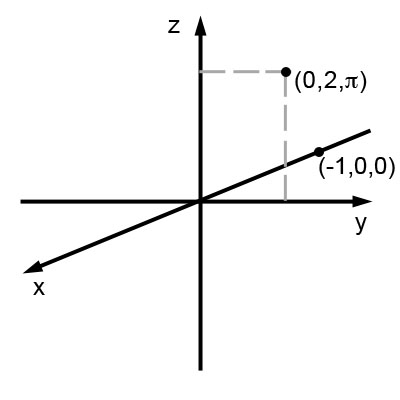
\includegraphics[width=0.45\textwidth]{ImgParticle.jpg}
  \end{center}
  \vspace{-20pt}
\end{figure}
% ~~~~~~~~~~~~~~~~~~~~~~~~~~~~~~~~~~~~~~~~~~~~~~~~~~~~~~~~~
\EEN % END OF SOLUTIONS


% ~~~~~~~~~~~~~~~~~~~~~~~~~~~~~~~~~~~~~~~~~~~~~~~~~~~~~~~~~
% ~~~~~~~~~~~~~~~~~~~~~~~~~~~~~~~~~~~~~~~~~~~~~~~~~~~~~~~~~

% QUESTIONS AND SOLUTIONS ON SIMILAR AND ORTHOGONAL MATRICES

%% -  -  -  -  -  -  -  -  -  -  -  -  -  -  -  -  -  -  -  -  -  -  -  -  -  -  -  -  -  -  
%\item 
%% QUESTION 5, MEDIUM
%%GPS: MMCA2c
%Let $A, B, C$ be three square matrices with the same dimensions.
%\begin{enumerate}
%\item Prove that if $A$ and $B$ are similar and $B$ and $C$ are similar then 
%$A$ and $C$ are similar.
%\item Let $x \in R$.  Prove that $A$ and $B + xI$ are similar whenever
%$A - xI$ and $B$ are similar.
%\item Suppose the system $A\mathbf{x} = \mathbf{b}$ has infinitely many solutions $x$ and that
%$A$ and $B$ are similar.  How many solutions can $B\mathbf{x} = \mathbf{b}$ have?
%\end{enumerate}
%
%% -  -  -  -  -  -  -  -  -  -  -  -  -  -  -  -  -  -  -  -  -  -  -  -  -  -  -  -  -  -  
%\item 
%% QUESTION 6, MEDIUM
%%GPS: MMCA2b 
%
%\begin{enumerate}
%\item Prove that, for any vectors $\mathbf{u}, \mathbf{v}$ and any orthogonal matrix $X$, $\mathbf{u} 
%\cdot \mathbf{v} = X\mathbf{u} \cdot X\mathbf{v}$
%\item Let $\mathbf{u}$ and $\mathbf{v}$ be two distinct vectors in $\R^{2}$.  Prove that, when 
%$X$ is an orthogonal matrix, the area of the parallelogram determined by $\mathbf{u}$ 
%and $\mathbf{v}$ is equal to the area of the parallelogram determined by $X\mathbf{u}$ and 
%$X\mathbf{v}$.
%\end{enumerate}

%
%\subsubsection*{(b)}
%
%Form the augmented matrix and apply row-reduction operations:
%
%\begin{align}
% \begin{bmatrix}
%  1 & 2 & -1 & 1 & 0 & 0 \\
%  2 & 5 & 0 & 0 & 1 & 0 \\
%  -3 & -5 & 4 & 0 & 0 & 1
% \end{bmatrix}&
% \nonumber \\
% \begin{bmatrix}
%  1 & 2 & -1 & 1 & 0 & 0 \\
%  0 & 1 & 2 & -2 & 1 & 0 \\
%  0 & 1 & 1 & 3 & 0 & 1
% \end{bmatrix}&
% \begin{array}{l}
%  R_2 \leftarrow R_2 - 2R_1 \\
%  R_3 \leftarrow R_3 + 3R_1
% \end{array}
% \nonumber \\
% \begin{bmatrix}
%  1 & 2 & -1 & 1 & 0 & 0 \\
%  0 & 1 & 2 & -2 & 1 & 0 \\
%  0 & 0 & -1 & 5 & -1 & 1
% \end{bmatrix}&
% \begin{array}{l}
%  R_3 \leftarrow R_3 - R_2
% \end{array}
% \nonumber \\
% \begin{bmatrix}
%  1 & 2 & -1 & 1 & 0 & 0 \\
%  0 & 1 & 0 & 8 & -1 & 2 \\
%  0 & 0 & 1 & -5 & 1 & -1
% \end{bmatrix}&
% \begin{array}{l}
%  R_2 \leftarrow R_2 + 2R_3 \\
%  R_3 \leftarrow -1 * R_3
% \end{array}
% \nonumber \\
% \begin{bmatrix}
%  1 & 0 & 0 & -20 & 3 & -5 \\
%  0 & 1 & 0 & 8 & -1 & 2 \\
%  0 & 0 & 1 & -5 & 1 & -1
% \end{bmatrix}&
% \begin{array}{l}
%  R_1 \leftarrow R_1 - 2R_2 + R_3
% \end{array}
% \nonumber
%\end{align}
%
%So the inverse matrix is
%\(\begin{bmatrix} -20 & 3 & -5 \\ 8 & -1 & 2 \\ -5 & 1 & -1 \end{bmatrix}\).
%
%\subsubsection*{(c)}
%
%The matrices $A_i$ are found by replacing the $i^{th}$ column of $A$ with
%the vector $b$.
%
%\begin{align*}
% A_1 &=
%  \begin{bmatrix}
%   1 & 2 & -1 \\
%   2 & 5 & 0 \\
%   -1 & -5 & 4
%  \end{bmatrix}, \det(A_1) = 20 - 16 + 5 = 9 \\
% A_2 &=
%  \begin{bmatrix}
%   1 & 1 & -1 \\
%   2 & 2 & 0 \\
%   -3 & -1 & 4
%  \end{bmatrix}, \det(A_2) = 8 - 8 - 4 = -4 \\
% A_3 &=
%  \begin{bmatrix}
%   1 & 2 & 1 \\
%   2 & 5 & 2 \\
%   -3 & -5 & -1
%  \end{bmatrix}, \det(A_3) = 5 - 8 + 5 = 2
%\end{align*}
%\subsection*{Question 5}
%
%\subsubsection*{(a)}
%Since $A$ and $B$ are similar and $B$ and $C$ are similar there exist
%matrices $S$ and $T$ such that $A = S^{-1}BS$ and $B = T^{-1}CT$; by
%substitution we see that $A = S^{-1}(T^{-1}CT)S = (TS)^{-1}C(TS)$.  If
%we set $U = TS$, then $A = U^{-1}CU$, so that A and C are similar.
%
%\subsubsection*{(b)}
%Since $A - xI$ and $B$ are similar there exists a square invertible matrix
%$C$ such that $C^{-1}(A - xI)C = B$.  By expanding the left-hand side of the
%equation we get $C^{-1}AC - C^{-1}xIC = B$.  However, since $x$ is a scalar,
%$C^{-1}xIC = xC^{-1}IC = xC^{-1}C = xI$, so that $C^{-1}AC - xI = B$.  By
%rearranging we see that $B + xI = C^{-1}AC$, so that $A$ and $B + xI$ are
%similar.
%
%\subsubsection*{(c)}
%Since $A$ and $B$ are similar, they have the same determinant.  The system
%$A\mathbf{x} = \mathbf{b}$ has infinitely many solutions, which, since $A$ is square, implies 
%that $A$ is not invertible, so that $\det(A) = \det(B) = 0$.  Therefore the 
%system $B\mathbf{x} = \mathbf{b}$ is either unsolvable or has infinitely many solutions.
%
%\subsection*{Question 6}
%
%\subsubsection*{(a)}
%Since $\mathbf{u} \cdot \mathbf{v} = \mathbf{u}^{T}\mathbf{v}$ for any vectors $\mathbf{u}, \mathbf{v}$ and $X^{T}X = I$, $X\mathbf{u}
%\cdot X\mathbf{v} = (X\mathbf{u})^{T}X\mathbf{v} = \mathbf{u}^{T}X^{T}X\mathbf{v} = \mathbf{u}^{T}\mathbf{v} = \mathbf{u} \cdot \mathbf{v}$.
%
%\subsubsection*{(b)}
%The area $area_{\mathbf{u},\mathbf{v}}$ of the parallelogram determined by $\mathbf{u}$ and $\mathbf{v}$ is given by the magnitude of the cross product $\mathbf{u} \times \mathbf{v}$:
%\[area_{\mathbf{u},\mathbf{v}} = ||\mathbf{u}||||\mathbf{v}|| \cdot |\sin(\theta_{\mathbf{u},\mathbf{v}})|\]
%where $\theta_{\mathbf{u},\mathbf{v}}$ is the angle between the vectors $\mathbf{u}, \mathbf{v}$.  Similarly,
%\[area_{X\mathbf{u},X\mathbf{v}}\ = ||X\mathbf{u}||||X\mathbf{v}|| \cdot |\sin(\theta_{X\mathbf{u},X\mathbf{v}})|\]
%Applying part (a) we see that $||X\mathbf{u}|| = \sqrt{X\mathbf{u} \cdot X\mathbf{u}} = \sqrt{\mathbf{u} \cdot \mathbf{u}} = ||\mathbf{u}||$ and $||X\mathbf{v}|| = ||\mathbf{v}||$.  Additionally,
%\begin{align*}
% \sin(\theta_{X\mathbf{u},X\mathbf{v}}) &= \sqrt{1 - \cos(\theta_{X\mathbf{u},X\mathbf{v}})^{2}} \\
% & = \sqrt{1 - (\dfrac{X\mathbf{u} \cdot X\mathbf{v}}{||X\mathbf{u}||||X\mathbf{v}||})^{2}} \\
% &= \sqrt{1 - (\dfrac{\mathbf{u} \cdot \mathbf{v}}{||\mathbf{u}||||\mathbf{v}||})^{2}} \\
% &= \sqrt{1 - \cos(\theta_{\mathbf{u},\mathbf{v}})^{2}} \\
% &= |\sin(\theta_{\mathbf{u},\mathbf{v}})|.
%\end{align*}
%
%Thus $area_{X\mathbf{u},X\mathbf{v}} = area_{\mathbf{u},\mathbf{v}}$.

